\documentclass[8pt,a4paper,compress]{beamer}

\usepackage{/home/siyer/lib/slides}

\title{The Harvey Mudd Miniature Machine (HMMM)}
\date{}

\begin{document}
\begin{frame}
\vfill
\titlepage
\end{frame}

\begin{frame}
\frametitle{Outline}
\tableofcontents
\end{frame}

\section{HMMM}
\begin{frame}[fragile]
\pause

A real computer must be able to
\begin{itemize}
\item Move information between registers and memory
\item Get data from the outside world
\item Print results
\item Make decisions
\end{itemize}

\pause
\bigskip

The Harvey Mudd Miniature Machine (HMMM) is organized as follows
\begin{itemize}
\item Both instructions and data are 16 bit wide
\item In addition to the program counter and instruction register, there are 16 registers named \lstinline{r0} through \lstinline{r15}
\item There are 256 memory locations
\end{itemize}

\pause
\bigskip

Instead of programming in binary (0's and 1's), we'll use assembly language, a programming language where each instruction has a symbolic representation

\pause
\bigskip

For example, to compute \lstinline{r3 = r1 + r2}, we'll write \lstinline{add r3 r1 r2}

\pause
\bigskip

We'll use a program\footnote{\href{http://www.swamiiyer.net/teaching/hmmm.zip}{http://www.swamiiyer.net/teaching/hmmm.zip} (command-line) or \href{http://shickey.github.io/HMMM.js}{http://shickey.github.io/HMMM.js} (online)} to convert the assembly language into 0's and 1's -- the machine language -- that the computer can execute
\end{frame}

\section{A Simple HMMM Program}

\begin{frame}[fragile]
\pause

\begin{framed}
\tiny triangle1.hmmm: Calculate the approximate area of a triangle.
\end{framed}

\begin{lstlisting}[language={}]
0    read    r1       # Get base b
1    read    r2       # Get height h
2    mul     r1 r1 r2 # b times h into r1
3    setn    r2 2
4    div     r1 r1 r2 # Divide by 2
5    write   r1
6    halt
\end{lstlisting}

\pause

\begin{lstlisting}[language={}]
$ python hmmmAssembler.py -f triangle1.hmmm -o triangle1.b

----------------------
| ASSEMBLY SUCCESSFUL |
----------------------

0 : 0000 0001 0000 0001        0    read    r1       # Get base b
1 : 0000 0010 0000 0001        1    read    r2       # Get height h
2 : 1000 0001 0001 0010        2    mul     r1 r1 r2 # b times h into r1
3 : 0001 0010 0000 0010        3    setn    r2 2
4 : 1001 0001 0001 0010        4    div     r1 r1 r2 # Divide by 2
5 : 0000 0001 0000 0010        5    write   r1
6 : 0000 0000 0000 0000        6    halt
\end{lstlisting}

\pause

\begin{lstlisting}[language={}]
$ python hmmmSimulator.py -f triangle1.b -n
4
5
10
\end{lstlisting}
\end{frame}

\section{Looping}
\begin{frame}[fragile]
\pause

Unconditional jump (\lstinline{jumpn N}): set program counter to address \lstinline{N}

\pause
\bigskip

\begin{framed}
\tiny triangle2.hmmm: Calculate the approximate areas of many triangles.
\end{framed}

\begin{lstlisting}[language={}]
0    read    r1       # Get base b
1    read    r2       # Get height h
2    mul     r1 r1 r2 # b times h into r1
3    setn    r2 2
4    div     r1 r1 r2 # Divide by 2
5    write   r1
6    jumpn   0
\end{lstlisting}

\pause

\begin{lstlisting}[language={}]
$ python hmmmSimulator.py -f triangle2.b -n
4
5
10
5
5
12
<ctrl-d>

End of input, halting program execution...
\end{lstlisting}
\end{frame}

\begin{frame}[fragile]
\pause

Conditional jump (\lstinline{jeqzn rX N}): if \lstinline{rX == 0}, then jump to line \lstinline{N}

\pause
\bigskip

\begin{framed}
\tiny triangle3.hmmm: Calculate the approximate areas of many triangles. Stop when a base or height of zero is given.
\end{framed}

\begin{lstlisting}[language={}]
0    read    r1       # Get base b
1    jeqzn   r1 9     # Jump to halt if base is zero
2    read    r2       # Get height h
3    jeqzn   r2 9     # Jump to halt if height is zero
4    mul     r1 r1 r2 # b times h into r1
5    setn    r2 2
6    div     r1 r1 r2 # Divide by 2
7    write   r1
8    jumpn   0
9    halt
\end{lstlisting}

\pause

\begin{lstlisting}[language={}]
$ python hmmmSimulator.py -f triangle3.b -n
4
5
10
5
5
12
0
\end{lstlisting}
\end{frame}

\section{Functions}

\begin{frame}[fragile]
\pause

Call a function (\lstinline{calln rX N}): copy the next address into \lstinline$rX$ and then jump to address \lstinline{N}; Return from a function (\lstinline{jumpr rX}): set program counter to address in \lstinline{rX}

\pause

\begin{framed}
\tiny square.hmmm: Calculate the square of a number $N$.
\end{framed}

\begin{lstlisting}[language={}]
0    read    r1    # Get N
1    calln   r14 5 # Calculate N^2 
2    write   r2    # Write answer
3    halt
4    nop           # Waste some space

# Square function. N is in r1. Result (N^2) is in r2. Return address is in r14.
5    mul     r2 r1 r1 # Calculate and store N^2 in r2
6    jumpr   r14      # Done; return to caller
\end{lstlisting}

\pause

\begin{lstlisting}[language={}]
$ python hmmmSimulator.py -f square.b -n
11
121
\end{lstlisting}
\end{frame}

\begin{frame}[fragile]
\pause

\begin{framed}
\tiny combinations.hmmm: Calculate $C(N, K)$ (aka $N$ choose $K$) defined as $C(N, K)=N!/(K!(N-K)!)$, where $N!$ ($N$ factorial) is defined as $N! = N \times (N-1) \times (N-2) \times \dots \times 2 \times 1$, with $0! = 1$.
\end{framed}

\begin{lstlisting}[language={}]
0    read    r3       # Get N
1    read    r4       # Get K
2    copy    r1 r3    # Calculate N!
3    calln   r14 15   # ...
4    copy    r5 r2    # Save N! as C(N, K)
5    copy    r1 r4    # Calculate K!
6    calln   r14 15   # ...
7    div     r5 r5 r2 # N!/K!
8    sub     r1 r3 r4 # Calculate (N - K)!
9    calln   r14 15   # ...
10   div     r5 r5 r2 # C(N, K)
11   write   r5       # Write answer
12   halt
13   nop              # Waste some space
14   nop

# Factorial function. N is in r1. Result is r2. Return address is in r14.
15    setn    r2 1     # Initial product
16    jeqzn   r1 20    # Quit if N has reached zero
17    mul     r2 r1 r2 # Update product
18    addn    r1 -1    # Decrement N
19    jumpn   16       # Back for more
20    jumpr   r14      # Done; return to caller
\end{lstlisting}

\pause

\begin{lstlisting}[language={}]
$ python hmmmSimulator.py -f combinations.b -n
5
2
10
\end{lstlisting}
\end{frame}

\begin{frame}[fragile]
\pause

\begin{minipage}{150pt}
\visible<2->{
Trace of the factorial function ($N=4$)
\begin{center}
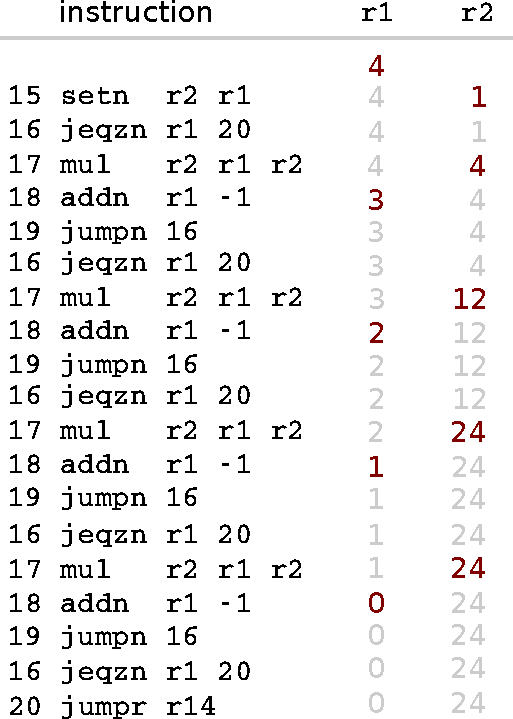
\includegraphics[scale=0.4]{./figures/hmmm_faciter_trace.pdf}
\end{center}
}
\end{minipage}
\begin{minipage}{150pt}%
\hfill
\visible<3->{
Trace of the program ($N=5, K=2$)
\begin{center}
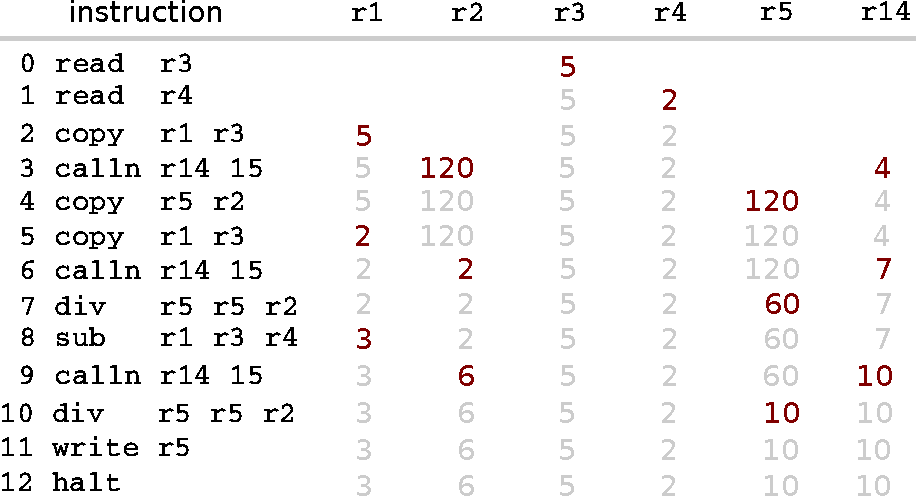
\includegraphics[scale=0.4]{./figures/hmmm_combinations_trace.pdf}
\end{center}
}
\end{minipage}
\end{frame}

\section{Recursion}

\begin{frame}[fragile]
\pause

A recursive function is a function that calls itself on smaller inputs, and has a base case. For example, the factorial function $N!$ can be expressed recursively as 
\[
N! = \begin{dcases*}
N(N-1)! & if $N > 0$, and \\
1       & if $N=0$
\end{dcases*}
\]

\pause
\bigskip

A stack is a storage mechanism (aka data structure) that remembers things and gives them back in reverse order

\pause
\bigskip

To implement a stack on a computer, we need a stack pointer, a register (\lstinline{r15} on HMMM) that holds the memory address of the top item on the stack

\pause
\bigskip

The code to push something, say the contents of \lstinline{r4}, atop the stack looks like this
\begin{lstlisting}[language={}]
addn   r15 1      # Point to a new location
storer r4 r15     # Store r4 on the stack
\end{lstlisting}

\pause
\bigskip

The code to recover the value atop the stack, say into \lstinline{r3}, looks like this
\begin{lstlisting}[language={}]
loadr r3 r15     # Load r3 from the stack
addn  r15 -1     # Point to new top of stack
\end{lstlisting}
\end{frame}

\begin{frame}[fragile]
\pause

\begin{framed}
\tiny factorial\_rec.hmmm: Calculate $N!$ recursively.
\end{framed}

\begin{lstlisting}[language={}]
0    setn    r15 100  # Initialize stack pointer
1    read    r2       # Get N
2    calln   r14 5    # Recursive function finds N!
3    write   r1       # Write result
4    halt

# Function to compute N! recursively. N is in r2. N! is in r1. 
5    jeqzn   r2 18     # Test for base case (0!)
6    addn    r15 1     # Save precious possessions
7    storer  r2 r15    # ...
8    addn    r15 1     # ...
9    storer  r14 r15   # ...
10   addn    r2 -1     # Calculate N - 1
11   calln   r14 5     # Call ourselves recursively to get (N - 1)!
12   loadr   r14 r15   # Recover precious possessions
13   addn    r15 -1    # ...
14   loadr   r2 r15    # ...
15   addn    r15 -1    # ...
16   mul     r1 r1 r2  # (N - 1)! times N
17   jumpr   r14       # Return to caller

# Base case: 0! is always 1
18   setn    r1 1
19   jumpr   r14       # Return to caller
\end{lstlisting}

\pause

\begin{lstlisting}[language={}]
$ python hmmmSimulator.py -f factorial_rec.b -n
5
120
\end{lstlisting}
\end{frame}

\begin{frame}[fragile]
\pause

Trace of the recursive factorial function ($N=3$)
\begin{center}
\visible<2->{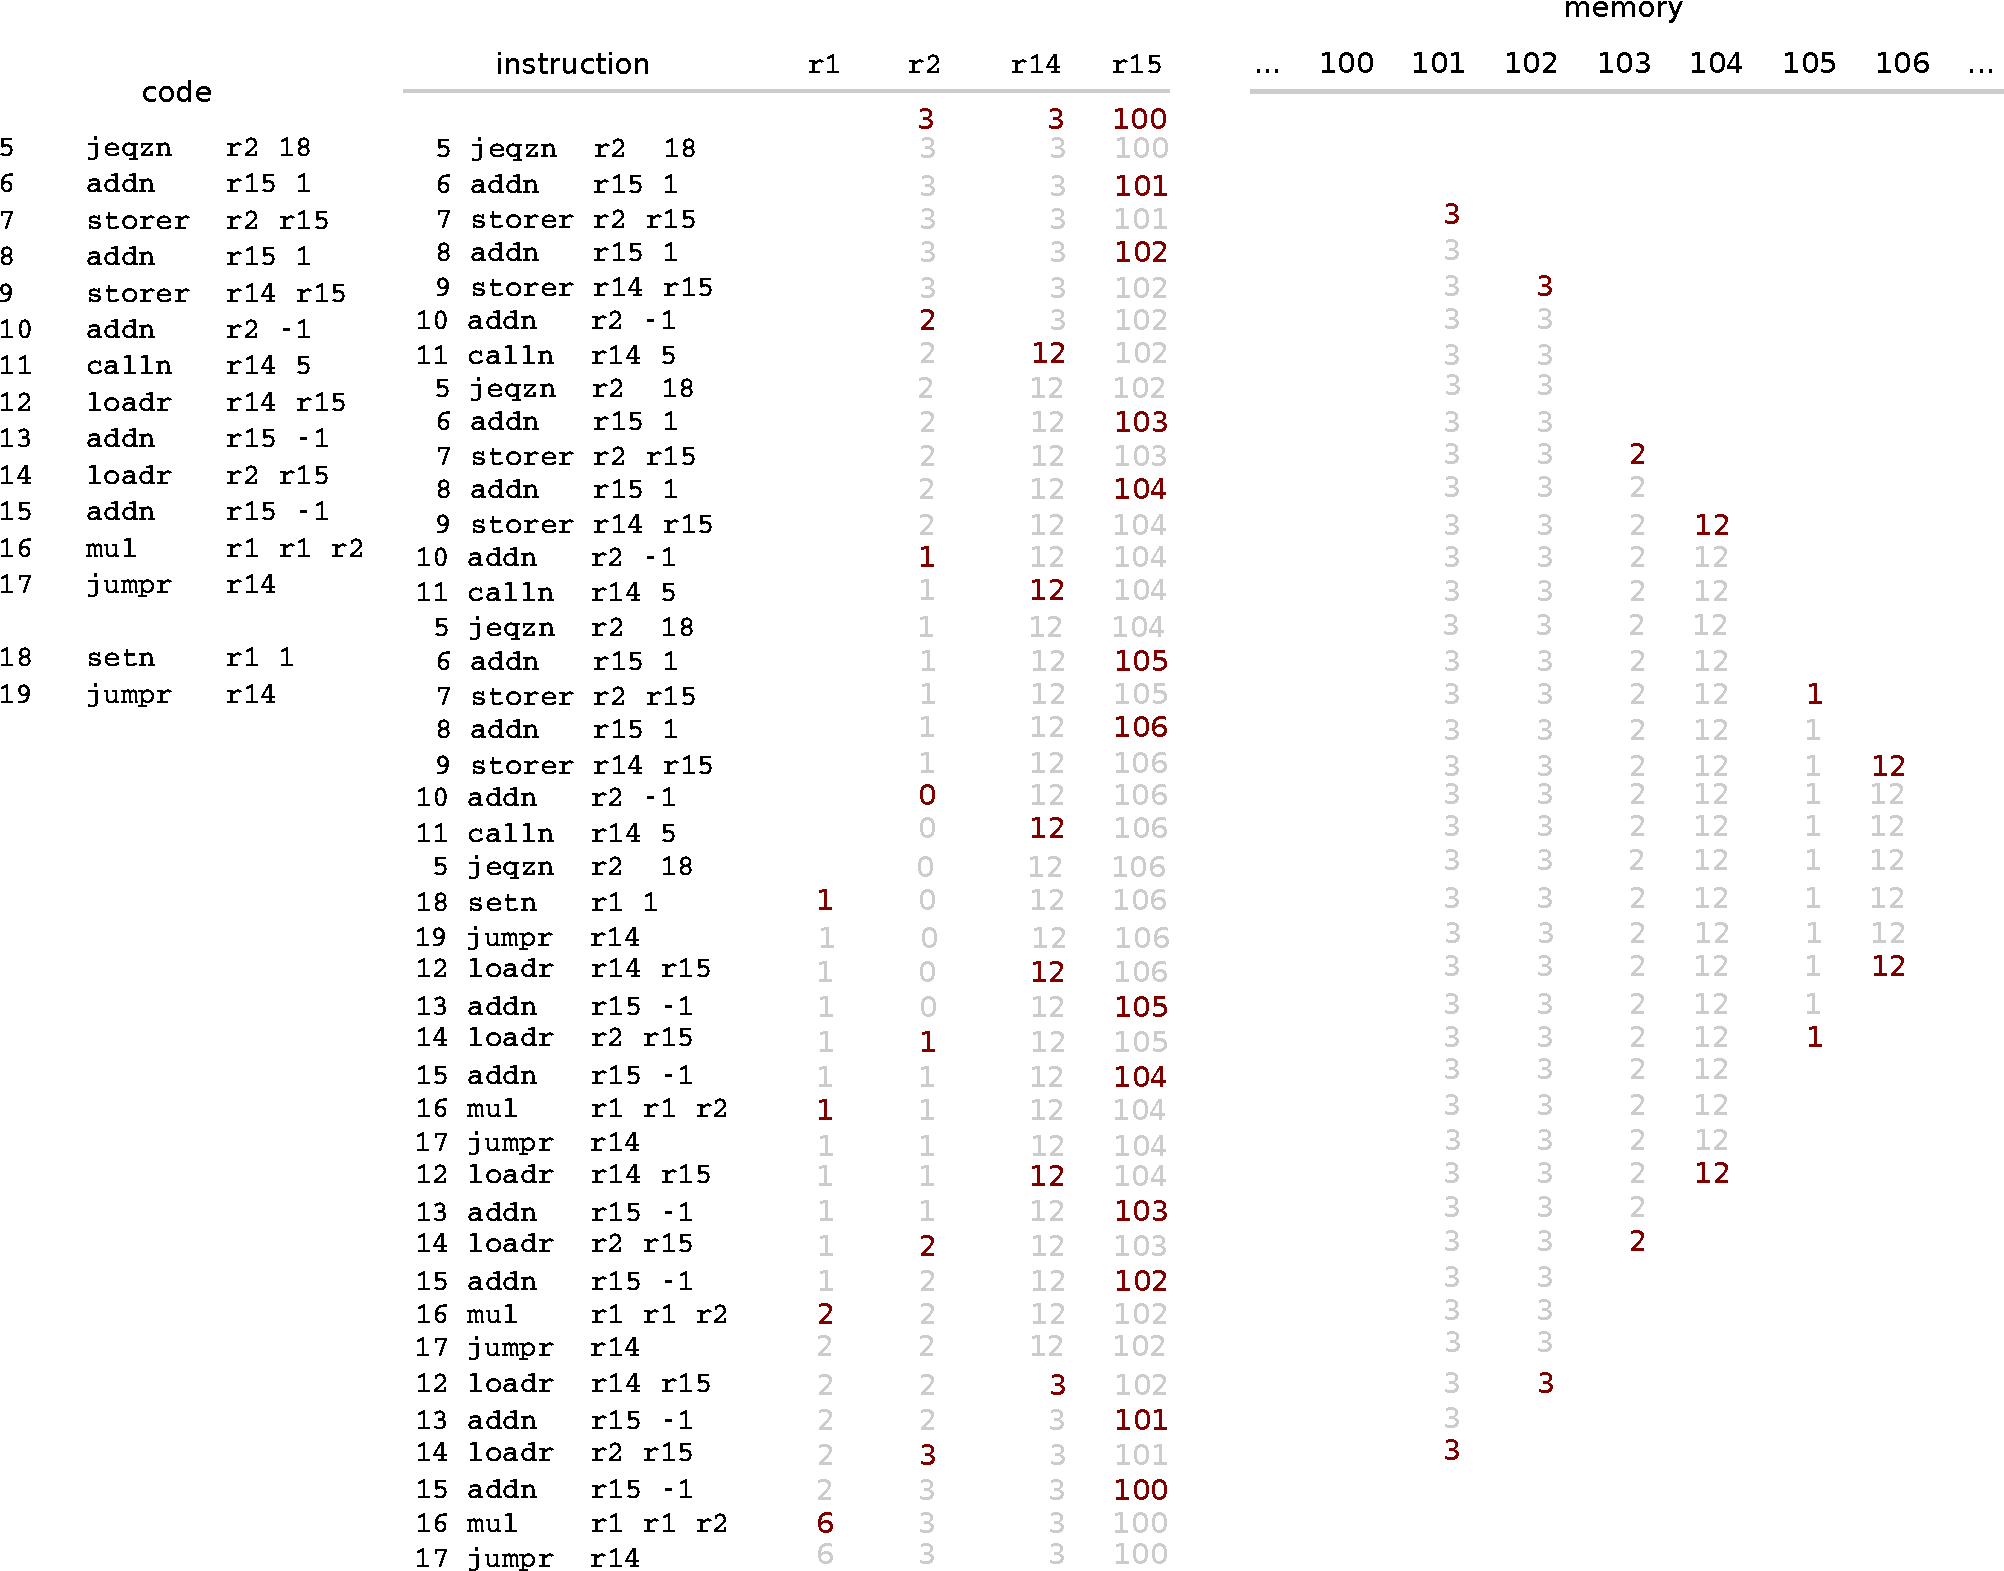
\includegraphics[scale=0.36]{./figures/hmmm_facrec_trace.pdf}}
\end{center}
\end{frame}

\section{HMMM Instruction Set}

\begin{frame}[fragile]
\pause

System instructions

\bigskip

\begin{tabular}{ll}
\lstinline$halt$ & stop \\
\lstinline$read rX$ & place user input in register \lstinline$rX$ \\
\lstinline$write rX$ & print contents of register \lstinline$rX$ \\
\lstinline$nop$ & do nothing
\end{tabular} 

\pause
\bigskip

Setting register data

\bigskip

\begin{tabular}{ll}
\lstinline$setn rX N$ & set register \lstinline$rX$ equal to the integer \lstinline$N$ (-128 to 127) \\
\lstinline$addn rX N$ & add integer \lstinline$N$ (-128 to 127) to register \lstinline$rX$ \\
\lstinline$copy rX rY$ & set \lstinline$rX = rY$
\end{tabular} 

\pause
\bigskip

Arithmetic

\bigskip

\begin{tabular}{ll}
\lstinline$add rX rY rZ$ & set \lstinline$rX = rY + rZ$ \\ 
\lstinline$sub rX rY rZ$ & set \lstinline$rX = rY - rZ$ \\ 
\lstinline$neg rX rY$ & set \lstinline$rX = -rY$ \\ 
\lstinline$mul rX rY rZ$ & set \lstinline$rX = rY * rZ$ \\ 
\lstinline$div rX rY rZ$ & set \lstinline$rX = rY / rZ$ (integer division; no remainder)\\ 
\lstinline$mod rX rY rZ$ & set \lstinline$rX = rY % rZ$ (returns the remainder of integer division) 
\end{tabular} 
\end{frame}

\begin{frame}[fragile]
\pause

Jumps

\bigskip

\begin{tabular}{ll}
\lstinline$jumpn N$ & set program counter to address \lstinline$N$ \\
\lstinline$jumpr rX$ & set program counter to address in \lstinline$rX$ \\
\lstinline$jeqzn rX N$ & if \lstinline$rX == 0$, then jump to line \lstinline$N$ \\
\lstinline$jnezn rX N$ & if \lstinline$rX != 0$, then jump to line \lstinline$N$ \\
\lstinline$jgtzn rX N$ & if \lstinline$rX > 0$, then jump to line \lstinline$N$ \\
\lstinline$jltzn rX N$ & if \lstinline$rX < 0$, then jump to line \lstinline$N$ \\
\lstinline$calln rX N$ & copy the next address into \lstinline$rX$ and then jump to address \lstinline$N$
\end{tabular} 

\pause
\bigskip

Interacting with memory

\bigskip

\begin{tabular}{ll}
\lstinline$loadn rX N$ & load register \lstinline$rX$ with the contents of address \lstinline$N$ \\
\lstinline$storen rX N$ & store contents of register \lstinline$rX$ into address \lstinline$N$ \\
\lstinline$loadr rX rY$ & load register \lstinline$rX$ with data from the address location held in register \lstinline$rY$ \\
\lstinline$storer rX rY$ & store contents of register \lstinline$rX$ into address held in register \lstinline$rY$ 
\end{tabular} 
\end{frame}
\end{document}
